\documentclass[border=1mm]{standalone}
\usepackage{tikz,tkz-euclide}
\usepackage{pgfplots}
\usetikzlibrary{arrows,calc,patterns,intersections}
\begin{document}


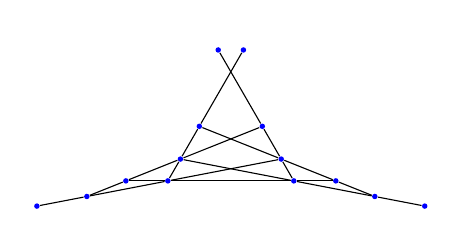
\begin{tikzpicture}[scale=0.8]

\tikzset{
    dot/.style={circle,inner sep=0.7pt,fill,label={\tiny #1},name=#1}}

\node at (-2.2,0) {~};    
\node at (2.2,0) {~};    
    
%\node[dot, fill=blue!10!red] (A) at (-1.4,0) {};
\node[dot, fill=blue] (B) at (-1,0) {};
\node[dot, fill=blue] (C) at (-0.8,{0.2*sqrt(3)}) {};
\node[dot, fill=blue] (D) at (-0.50,{0.50*sqrt(3)}) {};
\node[dot, fill=blue] (E) at (0.2,{1.2*sqrt(3)}) {};

%\node[dot, fill=blue!10!red] (F) at (1.4,0) {};
\node[dot, fill=blue] (G) at (1,0) {};
\node[dot, fill=blue] (H) at (0.8,{0.2*sqrt(3)}) {};
\node[dot, fill=blue] (I) at (0.50,{0.50*sqrt(3)}) {};
\node[dot, fill=blue] (J) at (-0.2,{1.2*sqrt(3)}) {};

%\node[dot, fill=blue!70!red] (D) at (-1,0) {};
%\node[dot, fill=blue!100!red] (E) at (-2,0) {};
%\node[dot, fill=blue!70!red] (F) at (1.5,{-0.5*sqrt(3)}) {};
%\node[dot, fill=blue!100!red] (G) at (2,{-1*sqrt(3)}) {};
%\node[dot, fill=blue!70!red] (H) at (1,{1*sqrt(3)}) {};
%\node[dot, fill=blue!100!red] (I) at (1.5,{1.5*sqrt(3)}) {};
%
\draw [name path=B--G, draw=none] (B) -- (G);
\draw [name path=D--I, draw=none] (D) -- (H);
\draw [name path=C--H, draw=none] (C) -- (I);
\draw [name path=B--H, draw=none] (B) -- (H);
\draw [name path=C--G, draw=none] (C) -- (G);

\node (P) at (-1,-0.4) {};
\node (Q) at (1,-0.4) {};

\draw [name path=P--Q, draw=none] (P) -- (Q);


%\draw [name path=C--D, draw=none] (C) -- (D);
%
\coordinate (Y) at (intersection of B--G and D--H);
\node[dot, fill=blue] (Y1) at (Y) {};

\coordinate (X) at (intersection of B--G and C--I);
\node[dot, fill=blue] (X1) at (X) {};


\coordinate (U) at (intersection of B--H and C--I);
\node[dot, fill=blue] (U1) at (U) {};

\coordinate (R) at (intersection of P--Q and B--H);
\node[dot, fill=blue] (R1) at (R) {};

\coordinate (V) at (intersection of C--G and D--H);
\node[dot, fill=blue] (V1) at (V) {};

\coordinate (S) at (intersection of P--Q and C--G);
\node[dot, fill=blue] (S1) at (S) {};

%
%\coordinate (Y) at (intersection of A--F and C--D);
%\node[dot, fill=blue!40!red] (Y1) at (Y) {};
%
%\coordinate (Z) at (intersection of B--H and C--D);
%\node[dot, fill=blue!40!red] (Z1) at (Z) {};
%
%

\draw (X1)--(B)--(G)--(Y1);
\draw (B) -- (C) -- (D) -- (E);
\draw (G) -- (H) -- (I) -- (J);

\draw (U1)--(X1)--(C)--(I);
\draw (V1)--(Y1)--(H)--(D);

\draw (R1)--(U1)--(B)--(H);
\draw (S1)--(V1)--(G)--(C);

%\draw (A) -- (D) -- (E);
%\draw (B) -- (F) -- (G);
%\draw (C) -- (H) -- (I);
%
%\draw (X1) -- (B) -- (Z1) -- (H);
%\draw (Y1) -- (A) -- (X1) -- (F);
%\draw (Z1) -- (C) -- (Y1) -- (D);

\end{tikzpicture}

\end{document}
